\documentclass[twoside]{book}

% Packages required by doxygen
\usepackage{fixltx2e}
\usepackage{calc}
\usepackage{doxygen}
\usepackage[export]{adjustbox} % also loads graphicx
\usepackage{graphicx}
\usepackage[utf8]{inputenc}
\usepackage{makeidx}
\usepackage{multicol}
\usepackage{multirow}
\PassOptionsToPackage{warn}{textcomp}
\usepackage{textcomp}
\usepackage[nointegrals]{wasysym}
\usepackage[table]{xcolor}

% NLS support packages
\usepackage[T2A]{fontenc}
\usepackage[russian]{babel}

% Font selection
\usepackage[T1]{fontenc}
\usepackage[scaled=.90]{helvet}
\usepackage{courier}
\usepackage{amssymb}
\usepackage{sectsty}
\renewcommand{\familydefault}{\sfdefault}
\allsectionsfont{%
  \fontseries{bc}\selectfont%
  \color{darkgray}%
}
\renewcommand{\DoxyLabelFont}{%
  \fontseries{bc}\selectfont%
  \color{darkgray}%
}
\newcommand{\+}{\discretionary{\mbox{\scriptsize$\hookleftarrow$}}{}{}}

% Page & text layout
\usepackage{geometry}
\geometry{%
  a4paper,%
  top=2.5cm,%
  bottom=2.5cm,%
  left=2.5cm,%
  right=2.5cm%
}
\tolerance=750
\hfuzz=15pt
\hbadness=750
\setlength{\emergencystretch}{15pt}
\setlength{\parindent}{0cm}
\setlength{\parskip}{3ex plus 2ex minus 2ex}
\makeatletter
\renewcommand{\paragraph}{%
  \@startsection{paragraph}{4}{0ex}{-1.0ex}{1.0ex}{%
    \normalfont\normalsize\bfseries\SS@parafont%
  }%
}
\renewcommand{\subparagraph}{%
  \@startsection{subparagraph}{5}{0ex}{-1.0ex}{1.0ex}{%
    \normalfont\normalsize\bfseries\SS@subparafont%
  }%
}
\makeatother

% Headers & footers
\usepackage{fancyhdr}
\pagestyle{fancyplain}
\fancyhead[LE]{\fancyplain{}{\bfseries\thepage}}
\fancyhead[CE]{\fancyplain{}{}}
\fancyhead[RE]{\fancyplain{}{\bfseries\leftmark}}
\fancyhead[LO]{\fancyplain{}{\bfseries\rightmark}}
\fancyhead[CO]{\fancyplain{}{}}
\fancyhead[RO]{\fancyplain{}{\bfseries\thepage}}
\fancyfoot[LE]{\fancyplain{}{}}
\fancyfoot[CE]{\fancyplain{}{}}
\fancyfoot[RE]{\fancyplain{}{\bfseries\scriptsize Создано системой Doxygen }}
\fancyfoot[LO]{\fancyplain{}{\bfseries\scriptsize Создано системой Doxygen }}
\fancyfoot[CO]{\fancyplain{}{}}
\fancyfoot[RO]{\fancyplain{}{}}
\renewcommand{\footrulewidth}{0.4pt}
\renewcommand{\chaptermark}[1]{%
  \markboth{#1}{}%
}
\renewcommand{\sectionmark}[1]{%
  \markright{\thesection\ #1}%
}

% Indices & bibliography
\usepackage{natbib}
\usepackage[titles]{tocloft}
\setcounter{tocdepth}{3}
\setcounter{secnumdepth}{5}
\makeindex

% Hyperlinks (required, but should be loaded last)
\usepackage{ifpdf}
\ifpdf
  \usepackage[pdftex,pagebackref=true]{hyperref}
\else
  \usepackage[ps2pdf,pagebackref=true]{hyperref}
\fi
\hypersetup{%
  colorlinks=true,%
  linkcolor=blue,%
  citecolor=blue,%
  unicode%
}

% Custom commands
\newcommand{\clearemptydoublepage}{%
  \newpage{\pagestyle{empty}\cleardoublepage}%
}

\usepackage{caption}
\captionsetup{labelsep=space,justification=centering,font={bf},singlelinecheck=off,skip=4pt,position=top}

%===== C O N T E N T S =====

\begin{document}

% Titlepage & ToC
\hypersetup{pageanchor=false,
             bookmarksnumbered=true,
             pdfencoding=unicode
            }
\pagenumbering{alph}
\begin{titlepage}
\vspace*{7cm}
\begin{center}%
{\Large data\+\_\+mining }\\
\vspace*{1cm}
{\large Создано системой Doxygen 1.8.13}\\
\end{center}
\end{titlepage}
\clearemptydoublepage
\pagenumbering{roman}
\tableofcontents
\clearemptydoublepage
\pagenumbering{arabic}
\hypersetup{pageanchor=true}

%--- Begin generated contents ---
\chapter{Автоматический веб-\/агрегатор для создания единой базы сертифицированных средств защиты информации}
\label{md_README}
\Hypertarget{md_README}

\begin{DoxyItemize}
\item Задание для летней практики 2017
\end{DoxyItemize}

Приложение -\/ консольное.

Чтобы запустить программу, необходимо написать следующие команды в терминале\+: 
\begin{DoxyCode}
git clone https://github.com/moskanka/DataMining
./get-reestr-mtmc.sh
\end{DoxyCode}


В процессе работы приложение заходит на \href{https://reestr.minsvyaz.ru/reestr/}{\tt сайт Единого реестра российских программ для ЭВМ и БД} и собирает оттуда необходимую информацию. Результаты записываются в файл {\ttfamily reestr.\+csv}, а так же выдаются прямо в консоль в {\ttfamily csv}-\/формате

Кодировка {\ttfamily csv}-\/файла\+: U\+T\+F-\/8 без B\+OM.

Ошибки выдаются в отдельном потоке -\/ {\ttfamily stderror}

{\bfseries Пример работы программы для одной из программ реестра\+:}


\begin{DoxyItemize}
\item Страница продукта\+: 
\item Выходной {\ttfamily csv}-\/файл\+: 
\item Если во входных данных нет искомого поля, то в него ставится значение по умолчанию, а если оно не оговоренно, то поле оставляется пустым.
\end{DoxyItemize}

{\bfseries Документация функций и классов\+:}

Чтобы открыть документацию к этому приложению необходимо написать в терминале (находясь в корневой папке проекта)\+: 
\begin{DoxyCode}
doxygen Doxyfile
cd html
gnome-open index.html
\end{DoxyCode}
 Так же можно вручную открыть файл {\ttfamily index.\+html} в удобном вам браузере. 
\chapter{Алфавитный указатель пространств имен}
\section{Пакеты}
Полный список документированных пакетов.\begin{DoxyCompactList}
\item\contentsline{section}{\hyperlink{namespaceget__urlslist}{get\+\_\+urlslist} \\*Модуль получения списка ссылок }{\pageref{namespaceget__urlslist}}{}
\item\contentsline{section}{\hyperlink{namespaceprint__results}{print\+\_\+results} \\*Модуль вывода результатов в консоль из файла {\bfseries {\itshape reestr.\+csv}} }{\pageref{namespaceprint__results}}{}
\item\contentsline{section}{\hyperlink{namespacereestr__spider}{reestr\+\_\+spider} \\*Паук для страницы реестра }{\pageref{namespacereestr__spider}}{}
\end{DoxyCompactList}

\chapter{Иерархический список классов}
\section{Иерархия классов}
Иерархия классов.\begin{DoxyCompactList}
\item \contentsline{section}{Csv\+Writer.\+Csv\+Writer}{\pageref{classCsvWriter_1_1CsvWriter}}{}
\item Item\begin{DoxyCompactList}
\item \contentsline{section}{data\+\_\+mining.\+items.\+Data\+Mining\+Item}{\pageref{classdata__mining_1_1items_1_1DataMiningItem}}{}
\end{DoxyCompactList}
\item object\begin{DoxyCompactList}
\item \contentsline{section}{data\+\_\+mining.\+middlewares.\+Data\+Mining\+Spider\+Middleware}{\pageref{classdata__mining_1_1middlewares_1_1DataMiningSpiderMiddleware}}{}
\item \contentsline{section}{data\+\_\+mining.\+pipelines.\+Data\+Mining\+Pipeline}{\pageref{classdata__mining_1_1pipelines_1_1DataMiningPipeline}}{}
\end{DoxyCompactList}
\item Spider\begin{DoxyCompactList}
\item \contentsline{section}{data\+\_\+mining.\+spiders.\+reestr\+\_\+spider.\+Reestr\+Spider}{\pageref{classdata__mining_1_1spiders_1_1reestr__spider_1_1ReestrSpider}}{}
\end{DoxyCompactList}
\item \contentsline{section}{Urls\+Receiver.\+Urls\+Receiver}{\pageref{classUrlsReceiver_1_1UrlsReceiver}}{}
\end{DoxyCompactList}

\chapter{Алфавитный указатель классов}
\section{Классы}
Классы с их кратким описанием.\begin{DoxyCompactList}
\item\contentsline{section}{\hyperlink{classCsvWriter_1_1CsvWriter}{Csv\+Writer.\+Csv\+Writer} \\*Класс, пишущий данные в {\ttfamily .csv} формат }{\pageref{classCsvWriter_1_1CsvWriter}}{}
\item\contentsline{section}{\hyperlink{classdata__mining_1_1items_1_1DataMiningItem}{data\+\_\+mining.\+items.\+Data\+Mining\+Item} }{\pageref{classdata__mining_1_1items_1_1DataMiningItem}}{}
\item\contentsline{section}{\hyperlink{classdata__mining_1_1pipelines_1_1DataMiningPipeline}{data\+\_\+mining.\+pipelines.\+Data\+Mining\+Pipeline} }{\pageref{classdata__mining_1_1pipelines_1_1DataMiningPipeline}}{}
\item\contentsline{section}{\hyperlink{classdata__mining_1_1middlewares_1_1DataMiningSpiderMiddleware}{data\+\_\+mining.\+middlewares.\+Data\+Mining\+Spider\+Middleware} }{\pageref{classdata__mining_1_1middlewares_1_1DataMiningSpiderMiddleware}}{}
\item\contentsline{section}{\hyperlink{classdata__mining_1_1spiders_1_1reestr__spider_1_1ReestrSpider}{data\+\_\+mining.\+spiders.\+reestr\+\_\+spider.\+Reestr\+Spider} \\*Класс паука }{\pageref{classdata__mining_1_1spiders_1_1reestr__spider_1_1ReestrSpider}}{}
\item\contentsline{section}{\hyperlink{classUrlsReceiver_1_1UrlsReceiver}{Urls\+Receiver.\+Urls\+Receiver} \\*Получатель списка ссылок }{\pageref{classUrlsReceiver_1_1UrlsReceiver}}{}
\end{DoxyCompactList}

\chapter{Пространства имен}
\input{namespaceget__urlslist}
\input{namespaceprint__results}
\hypertarget{namespacereestr__spider}{}\section{Пространство имен reestr\+\_\+spider}
\label{namespacereestr__spider}\index{reestr\+\_\+spider@{reestr\+\_\+spider}}


Паук для страницы реестра  


\subsection*{Классы}
\begin{DoxyCompactItemize}
\item 
class \hyperlink{classreestr__spider_1_1ReestrSpider}{Reestr\+Spider}
\begin{DoxyCompactList}\small\item\em Класс паука \end{DoxyCompactList}\end{DoxyCompactItemize}
\subsection*{Функции}
\begin{DoxyCompactItemize}
\item 
def \hyperlink{namespacereestr__spider_a3ea2fa58027d32fc4f77d612777789fe}{get\+\_\+urls} ()
\begin{DoxyCompactList}\small\item\em Функция, получающая список ссылок \end{DoxyCompactList}\end{DoxyCompactItemize}
\subsection*{Переменные}
\begin{DoxyCompactItemize}
\item 
\mbox{\Hypertarget{namespacereestr__spider_a91a73e9f55aafc7333ccec0b50381179}\label{namespacereestr__spider_a91a73e9f55aafc7333ccec0b50381179}} 
\hyperlink{namespacereestr__spider_a91a73e9f55aafc7333ccec0b50381179}{csv\+\_\+worker} = cw.\+Csv\+Writer()
\begin{DoxyCompactList}\small\item\em Объект класса Csv\+Writer Объект класса Csv\+Writer, с помощью которого класс \hyperlink{classreestr__spider_1_1ReestrSpider}{Reestr\+Spider} сохраняет полученные со страниц реестра данные в формате .csv. \end{DoxyCompactList}\end{DoxyCompactItemize}


\subsection{Подробное описание}
Паук для страницы реестра 

\subsection{Функции}
\mbox{\Hypertarget{namespacereestr__spider_a3ea2fa58027d32fc4f77d612777789fe}\label{namespacereestr__spider_a3ea2fa58027d32fc4f77d612777789fe}} 
\index{reestr\+\_\+spider@{reestr\+\_\+spider}!get\+\_\+urls@{get\+\_\+urls}}
\index{get\+\_\+urls@{get\+\_\+urls}!reestr\+\_\+spider@{reestr\+\_\+spider}}
\subsubsection{\texorpdfstring{get\+\_\+urls()}{get\_urls()}}
{\footnotesize\ttfamily def reestr\+\_\+spider.\+get\+\_\+urls (\begin{DoxyParamCaption}{ }\end{DoxyParamCaption})}



Функция, получающая список ссылок 

\begin{DoxyReturn}{Возвращает}
Список ссылок на страницы реестра, которые считываются из файла \textquotesingle{}urls.\+txt\textquotesingle{} 
\end{DoxyReturn}

\chapter{Классы}
\hypertarget{classCsvWriter_1_1CsvWriter}{}\section{Класс Csv\+Writer.\+Csv\+Writer}
\label{classCsvWriter_1_1CsvWriter}\index{Csv\+Writer.\+Csv\+Writer@{Csv\+Writer.\+Csv\+Writer}}


Класс, пишущий данные в {\ttfamily .csv} формат  


\subsection*{Открытые члены}
\begin{DoxyCompactItemize}
\item 
def \hyperlink{classCsvWriter_1_1CsvWriter_aa46f0b7a79563167fff4906843f3ad00}{\+\_\+\+\_\+init\+\_\+\+\_\+} (self)
\begin{DoxyCompactList}\small\item\em Конструктор \end{DoxyCompactList}\item 
def \hyperlink{classCsvWriter_1_1CsvWriter_a82a1a0b729344761424248f4e8357abf}{make\+\_\+start\+\_\+pack} (self)
\begin{DoxyCompactList}\small\item\em Заполняет переменные строк начальными стандартными данными \end{DoxyCompactList}\item 
def \hyperlink{classCsvWriter_1_1CsvWriter_aa15d806d5045226507d60be0b8e25fab}{add} (self, field\+\_\+id, value)
\begin{DoxyCompactList}\small\item\em Метод, добавляющий строку с данными \end{DoxyCompactList}\item 
def \hyperlink{classCsvWriter_1_1CsvWriter_a9ce130eed2e7aac0e223740206519836}{save\+\_\+session} (self)
\begin{DoxyCompactList}\small\item\em Сохранение данных про данную программу из реестра \end{DoxyCompactList}\end{DoxyCompactItemize}
\subsection*{Открытые статические члены}
\begin{DoxyCompactItemize}
\item 
def \hyperlink{classCsvWriter_1_1CsvWriter_a3c0708fb8d6c9a9a72eee1027b4a336e}{field\+\_\+type} (value)
\begin{DoxyCompactList}\small\item\em Метод, определяющий тип поля \end{DoxyCompactList}\end{DoxyCompactItemize}
\subsection*{Открытые атрибуты}
\begin{DoxyCompactItemize}
\item 
\mbox{\Hypertarget{classCsvWriter_1_1CsvWriter_a7900ae93bb5ed7cf1896056c3f58e1d5}\label{classCsvWriter_1_1CsvWriter_a7900ae93bb5ed7cf1896056c3f58e1d5}} 
\hyperlink{classCsvWriter_1_1CsvWriter_a7900ae93bb5ed7cf1896056c3f58e1d5}{id\+\_\+row}
\begin{DoxyCompactList}\small\item\em Строка таблицы -\/ {\itshape {\bfseries Регистрационный номер}} \end{DoxyCompactList}\item 
\mbox{\Hypertarget{classCsvWriter_1_1CsvWriter_ae5e24b59bde75109c2ea93bbf7e69ddb}\label{classCsvWriter_1_1CsvWriter_ae5e24b59bde75109c2ea93bbf7e69ddb}} 
\hyperlink{classCsvWriter_1_1CsvWriter_ae5e24b59bde75109c2ea93bbf7e69ddb}{title\+\_\+row}
\begin{DoxyCompactList}\small\item\em Строка таблицы -\/ {\itshape {\bfseries Название продукта}} \end{DoxyCompactList}\item 
\mbox{\Hypertarget{classCsvWriter_1_1CsvWriter_a112e224f259e3bcce3a81540b195857d}\label{classCsvWriter_1_1CsvWriter_a112e224f259e3bcce3a81540b195857d}} 
\hyperlink{classCsvWriter_1_1CsvWriter_a112e224f259e3bcce3a81540b195857d}{alt\+\_\+title\+\_\+row}
\begin{DoxyCompactList}\small\item\em Строка таблицы -\/ {\itshape {\bfseries Другие названия продукта}} \end{DoxyCompactList}\item 
\mbox{\Hypertarget{classCsvWriter_1_1CsvWriter_a9b4127aab4f2b7db22c1f1d6fb86ac2c}\label{classCsvWriter_1_1CsvWriter_a9b4127aab4f2b7db22c1f1d6fb86ac2c}} 
\hyperlink{classCsvWriter_1_1CsvWriter_a9b4127aab4f2b7db22c1f1d6fb86ac2c}{date\+\_\+row}
\begin{DoxyCompactList}\small\item\em Строка таблицы -\/ {\itshape {\bfseries Дата геристрации в реестре}} \end{DoxyCompactList}\item 
\mbox{\Hypertarget{classCsvWriter_1_1CsvWriter_ace04c34812ce9261cafeda325461fa56}\label{classCsvWriter_1_1CsvWriter_ace04c34812ce9261cafeda325461fa56}} 
\hyperlink{classCsvWriter_1_1CsvWriter_ace04c34812ce9261cafeda325461fa56}{type\+\_\+app\+\_\+row}
\begin{DoxyCompactList}\small\item\em Строка таблицы -\/ {\itshape {\bfseries Класс ПО}} \end{DoxyCompactList}\item 
\mbox{\Hypertarget{classCsvWriter_1_1CsvWriter_afe13d494adecea2d49774a94ed04d0c5}\label{classCsvWriter_1_1CsvWriter_afe13d494adecea2d49774a94ed04d0c5}} 
\hyperlink{classCsvWriter_1_1CsvWriter_afe13d494adecea2d49774a94ed04d0c5}{app\+\_\+title\+\_\+row}
\begin{DoxyCompactList}\small\item\em Строка таблицы -\/ {\itshape {\bfseries Наименование заявителя}} \end{DoxyCompactList}\item 
\mbox{\Hypertarget{classCsvWriter_1_1CsvWriter_ae0f4694ebe36ba7b3b7446801b72415d}\label{classCsvWriter_1_1CsvWriter_ae0f4694ebe36ba7b3b7446801b72415d}} 
\hyperlink{classCsvWriter_1_1CsvWriter_ae0f4694ebe36ba7b3b7446801b72415d}{app\+\_\+url\+\_\+row}
\begin{DoxyCompactList}\small\item\em Строка таблицы -\/ {\itshape {\bfseries Сайт проивзодителя}} \end{DoxyCompactList}\item 
\mbox{\Hypertarget{classCsvWriter_1_1CsvWriter_ab40819d24b9d9d72f273a2663d9543ea}\label{classCsvWriter_1_1CsvWriter_ab40819d24b9d9d72f273a2663d9543ea}} 
\hyperlink{classCsvWriter_1_1CsvWriter_ab40819d24b9d9d72f273a2663d9543ea}{session\+\_\+rows}
\begin{DoxyCompactList}\small\item\em Массив всех строк таблицы, соответствующих одному продукту \end{DoxyCompactList}\item 
\mbox{\Hypertarget{classCsvWriter_1_1CsvWriter_a6550d0a2ebdbea5598569e289ec4c6b3}\label{classCsvWriter_1_1CsvWriter_a6550d0a2ebdbea5598569e289ec4c6b3}} 
\hyperlink{classCsvWriter_1_1CsvWriter_a6550d0a2ebdbea5598569e289ec4c6b3}{file}
\begin{DoxyCompactList}\small\item\em Файл, куда производится запись всех данных -\/ {\itshape {\bfseries reestr.\+csv}} \end{DoxyCompactList}\item 
\mbox{\Hypertarget{classCsvWriter_1_1CsvWriter_a46802d46472b31cff937ba338ec9aa31}\label{classCsvWriter_1_1CsvWriter_a46802d46472b31cff937ba338ec9aa31}} 
\hyperlink{classCsvWriter_1_1CsvWriter_a46802d46472b31cff937ba338ec9aa31}{writer}
\begin{DoxyCompactList}\small\item\em Объект класса {\itshape {\bfseries csv.\+writer}}, с помощью которого производится запись данных в {\itshape {\bfseries self.\+file}} \end{DoxyCompactList}\end{DoxyCompactItemize}


\subsection{Подробное описание}
Класс, пишущий данные в {\ttfamily .csv} формат 

Каждая программа из реестра записывается в файл {\itshape {\bfseries reestr.\+csv}}, и ее описание выглядит следующим образом\+:  

\subsection{Конструктор(ы)}
\mbox{\Hypertarget{classCsvWriter_1_1CsvWriter_aa46f0b7a79563167fff4906843f3ad00}\label{classCsvWriter_1_1CsvWriter_aa46f0b7a79563167fff4906843f3ad00}} 
\index{Csv\+Writer\+::\+Csv\+Writer@{Csv\+Writer\+::\+Csv\+Writer}!\+\_\+\+\_\+init\+\_\+\+\_\+@{\+\_\+\+\_\+init\+\_\+\+\_\+}}
\index{\+\_\+\+\_\+init\+\_\+\+\_\+@{\+\_\+\+\_\+init\+\_\+\+\_\+}!Csv\+Writer\+::\+Csv\+Writer@{Csv\+Writer\+::\+Csv\+Writer}}
\subsubsection{\texorpdfstring{\+\_\+\+\_\+init\+\_\+\+\_\+()}{\_\_init\_\_()}}
{\footnotesize\ttfamily def Csv\+Writer.\+Csv\+Writer.\+\_\+\+\_\+init\+\_\+\+\_\+ (\begin{DoxyParamCaption}\item[{}]{self }\end{DoxyParamCaption})}



Конструктор 

Все переменные, соответствующие строкам таблицы, заполняются функцией \hyperlink{classCsvWriter_1_1CsvWriter_a82a1a0b729344761424248f4e8357abf}{make\+\_\+start\+\_\+pack()} 

\subsection{Методы}
\mbox{\Hypertarget{classCsvWriter_1_1CsvWriter_aa15d806d5045226507d60be0b8e25fab}\label{classCsvWriter_1_1CsvWriter_aa15d806d5045226507d60be0b8e25fab}} 
\index{Csv\+Writer\+::\+Csv\+Writer@{Csv\+Writer\+::\+Csv\+Writer}!add@{add}}
\index{add@{add}!Csv\+Writer\+::\+Csv\+Writer@{Csv\+Writer\+::\+Csv\+Writer}}
\subsubsection{\texorpdfstring{add()}{add()}}
{\footnotesize\ttfamily def Csv\+Writer.\+Csv\+Writer.\+add (\begin{DoxyParamCaption}\item[{}]{self,  }\item[{}]{field\+\_\+id,  }\item[{}]{value }\end{DoxyParamCaption})}



Метод, добавляющий строку с данными 


\begin{DoxyParams}{Аргументы}
{\em self} & \\
\hline
{\em field\+\_\+id} & Идентификатор поля \\
\hline
{\em value} & Значение поля \\
\hline
\end{DoxyParams}
\mbox{\Hypertarget{classCsvWriter_1_1CsvWriter_a3c0708fb8d6c9a9a72eee1027b4a336e}\label{classCsvWriter_1_1CsvWriter_a3c0708fb8d6c9a9a72eee1027b4a336e}} 
\index{Csv\+Writer\+::\+Csv\+Writer@{Csv\+Writer\+::\+Csv\+Writer}!field\+\_\+type@{field\+\_\+type}}
\index{field\+\_\+type@{field\+\_\+type}!Csv\+Writer\+::\+Csv\+Writer@{Csv\+Writer\+::\+Csv\+Writer}}
\subsubsection{\texorpdfstring{field\+\_\+type()}{field\_type()}}
{\footnotesize\ttfamily def Csv\+Writer.\+Csv\+Writer.\+field\+\_\+type (\begin{DoxyParamCaption}\item[{}]{value }\end{DoxyParamCaption})\hspace{0.3cm}{\ttfamily [static]}}



Метод, определяющий тип поля 

Если длина содержимого больше 15 символов, то тип поля будет {\itshape {\bfseries Длинный текст}}, иначе -\/ {\itshape {\bfseries Текст}} \mbox{\Hypertarget{classCsvWriter_1_1CsvWriter_a82a1a0b729344761424248f4e8357abf}\label{classCsvWriter_1_1CsvWriter_a82a1a0b729344761424248f4e8357abf}} 
\index{Csv\+Writer\+::\+Csv\+Writer@{Csv\+Writer\+::\+Csv\+Writer}!make\+\_\+start\+\_\+pack@{make\+\_\+start\+\_\+pack}}
\index{make\+\_\+start\+\_\+pack@{make\+\_\+start\+\_\+pack}!Csv\+Writer\+::\+Csv\+Writer@{Csv\+Writer\+::\+Csv\+Writer}}
\subsubsection{\texorpdfstring{make\+\_\+start\+\_\+pack()}{make\_start\_pack()}}
{\footnotesize\ttfamily def Csv\+Writer.\+Csv\+Writer.\+make\+\_\+start\+\_\+pack (\begin{DoxyParamCaption}\item[{}]{self }\end{DoxyParamCaption})}



Заполняет переменные строк начальными стандартными данными 

Таблица для записываемой программы из реестра после выполнения этой функции выглядит так\+:  \mbox{\Hypertarget{classCsvWriter_1_1CsvWriter_a9ce130eed2e7aac0e223740206519836}\label{classCsvWriter_1_1CsvWriter_a9ce130eed2e7aac0e223740206519836}} 
\index{Csv\+Writer\+::\+Csv\+Writer@{Csv\+Writer\+::\+Csv\+Writer}!save\+\_\+session@{save\+\_\+session}}
\index{save\+\_\+session@{save\+\_\+session}!Csv\+Writer\+::\+Csv\+Writer@{Csv\+Writer\+::\+Csv\+Writer}}
\subsubsection{\texorpdfstring{save\+\_\+session()}{save\_session()}}
{\footnotesize\ttfamily def Csv\+Writer.\+Csv\+Writer.\+save\+\_\+session (\begin{DoxyParamCaption}\item[{}]{self }\end{DoxyParamCaption})}



Сохранение данных про данную программу из реестра 

Все строки записываются в массив \hyperlink{classCsvWriter_1_1CsvWriter_ab40819d24b9d9d72f273a2663d9543ea}{session\+\_\+rows}, после чего записываются в файл {\itshape {\bfseries reestr.\+csv}}, а затем обнуляются функцией \hyperlink{classCsvWriter_1_1CsvWriter_a82a1a0b729344761424248f4e8357abf}{make\+\_\+start\+\_\+pack()}, чтобы можно было начать обработку последующей программы из реестра. 

Объявления и описания членов класса находятся в файле\+:\begin{DoxyCompactItemize}
\item 
Csv\+Writer.\+py\end{DoxyCompactItemize}

\hypertarget{classitems_1_1DataMiningItem}{}\section{Класс items.\+Data\+Mining\+Item}
\label{classitems_1_1DataMiningItem}\index{items.\+Data\+Mining\+Item@{items.\+Data\+Mining\+Item}}
Граф наследования\+:items.\+Data\+Mining\+Item\+:\begin{figure}[H]
\begin{center}
\leavevmode
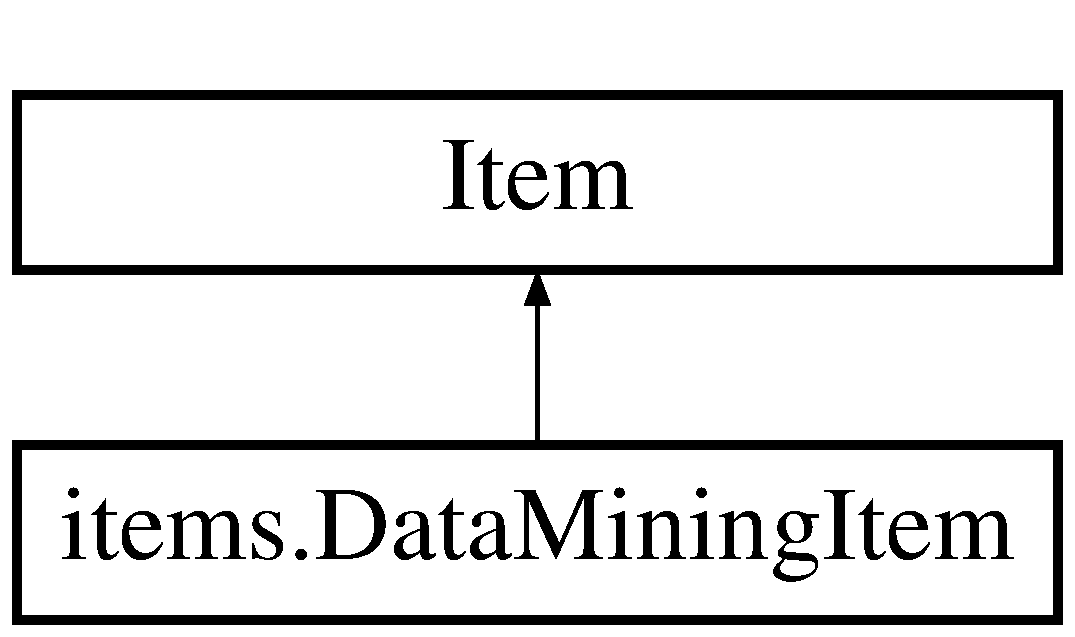
\includegraphics[height=2.000000cm]{classitems_1_1DataMiningItem}
\end{center}
\end{figure}


Объявления и описания членов класса находятся в файле\+:\begin{DoxyCompactItemize}
\item 
data\+\_\+mining/items.\+py\end{DoxyCompactItemize}

\hypertarget{classpipelines_1_1DataMiningPipeline}{}\section{Класс pipelines.\+Data\+Mining\+Pipeline}
\label{classpipelines_1_1DataMiningPipeline}\index{pipelines.\+Data\+Mining\+Pipeline@{pipelines.\+Data\+Mining\+Pipeline}}
Граф наследования\+:pipelines.\+Data\+Mining\+Pipeline\+:\begin{figure}[H]
\begin{center}
\leavevmode
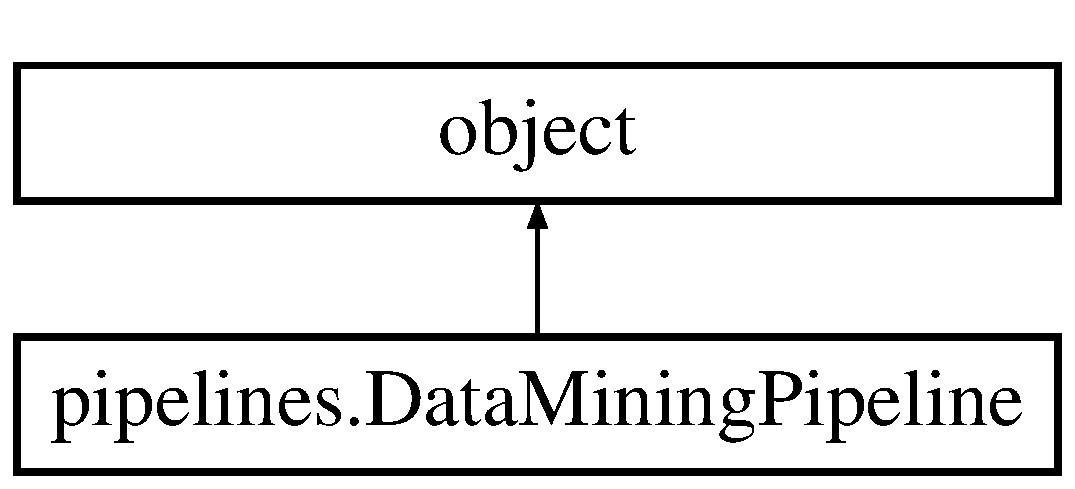
\includegraphics[height=2.000000cm]{classpipelines_1_1DataMiningPipeline}
\end{center}
\end{figure}
\subsection*{Открытые члены}
\begin{DoxyCompactItemize}
\item 
\mbox{\Hypertarget{classpipelines_1_1DataMiningPipeline_aae5a52dc0c5f5cb2d5ffc518a185a48c}\label{classpipelines_1_1DataMiningPipeline_aae5a52dc0c5f5cb2d5ffc518a185a48c}} 
def {\bfseries process\+\_\+item} (self, item, spider)
\end{DoxyCompactItemize}


Объявления и описания членов класса находятся в файле\+:\begin{DoxyCompactItemize}
\item 
data\+\_\+mining/pipelines.\+py\end{DoxyCompactItemize}

\hypertarget{classmiddlewares_1_1DataMiningSpiderMiddleware}{}\section{Класс middlewares.\+Data\+Mining\+Spider\+Middleware}
\label{classmiddlewares_1_1DataMiningSpiderMiddleware}\index{middlewares.\+Data\+Mining\+Spider\+Middleware@{middlewares.\+Data\+Mining\+Spider\+Middleware}}
Граф наследования\+:middlewares.\+Data\+Mining\+Spider\+Middleware\+:\begin{figure}[H]
\begin{center}
\leavevmode
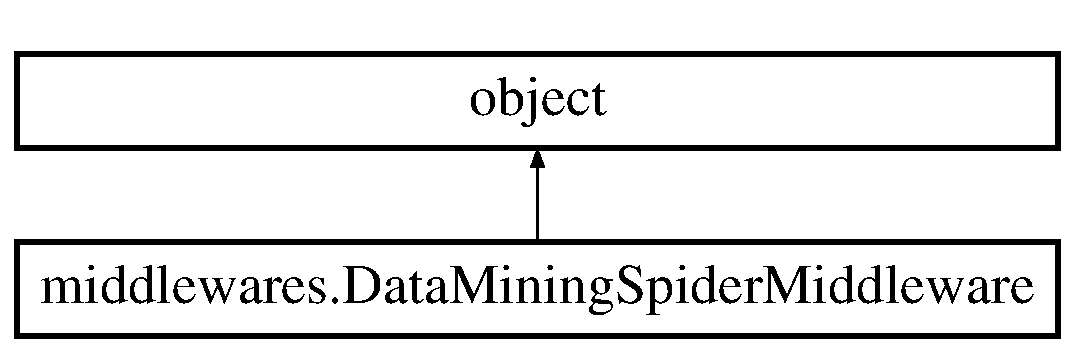
\includegraphics[height=2.000000cm]{classmiddlewares_1_1DataMiningSpiderMiddleware}
\end{center}
\end{figure}
\subsection*{Открытые члены}
\begin{DoxyCompactItemize}
\item 
\mbox{\Hypertarget{classmiddlewares_1_1DataMiningSpiderMiddleware_ab6e371356ca5c53fa4b062bfc212608b}\label{classmiddlewares_1_1DataMiningSpiderMiddleware_ab6e371356ca5c53fa4b062bfc212608b}} 
def {\bfseries from\+\_\+crawler} (cls, crawler)
\item 
\mbox{\Hypertarget{classmiddlewares_1_1DataMiningSpiderMiddleware_a3a8b7b75911f5dd8ed5ff651a8e8e973}\label{classmiddlewares_1_1DataMiningSpiderMiddleware_a3a8b7b75911f5dd8ed5ff651a8e8e973}} 
def {\bfseries process\+\_\+spider\+\_\+input} (self, response, spider)
\item 
\mbox{\Hypertarget{classmiddlewares_1_1DataMiningSpiderMiddleware_a08999e10ad91f078c5d41d24676895b0}\label{classmiddlewares_1_1DataMiningSpiderMiddleware_a08999e10ad91f078c5d41d24676895b0}} 
def {\bfseries process\+\_\+spider\+\_\+output} (self, response, result, spider)
\item 
\mbox{\Hypertarget{classmiddlewares_1_1DataMiningSpiderMiddleware_a1d361f268988e8d57f5a8a838a29b8b4}\label{classmiddlewares_1_1DataMiningSpiderMiddleware_a1d361f268988e8d57f5a8a838a29b8b4}} 
def {\bfseries process\+\_\+spider\+\_\+exception} (self, response, exception, spider)
\item 
\mbox{\Hypertarget{classmiddlewares_1_1DataMiningSpiderMiddleware_a54b198f045af39cc060f003c669a9b76}\label{classmiddlewares_1_1DataMiningSpiderMiddleware_a54b198f045af39cc060f003c669a9b76}} 
def {\bfseries process\+\_\+start\+\_\+requests} (self, start\+\_\+requests, spider)
\item 
\mbox{\Hypertarget{classmiddlewares_1_1DataMiningSpiderMiddleware_a48cfdfe4488bdb5059821813230f02df}\label{classmiddlewares_1_1DataMiningSpiderMiddleware_a48cfdfe4488bdb5059821813230f02df}} 
def {\bfseries spider\+\_\+opened} (self, spider)
\end{DoxyCompactItemize}


Объявления и описания членов класса находятся в файле\+:\begin{DoxyCompactItemize}
\item 
data\+\_\+mining/middlewares.\+py\end{DoxyCompactItemize}

\hypertarget{classreestr__spider_1_1ReestrSpider}{}\section{Класс reestr\+\_\+spider.\+Reestr\+Spider}
\label{classreestr__spider_1_1ReestrSpider}\index{reestr\+\_\+spider.\+Reestr\+Spider@{reestr\+\_\+spider.\+Reestr\+Spider}}


Класс паука  


Граф наследования\+:reestr\+\_\+spider.\+Reestr\+Spider\+:\begin{figure}[H]
\begin{center}
\leavevmode
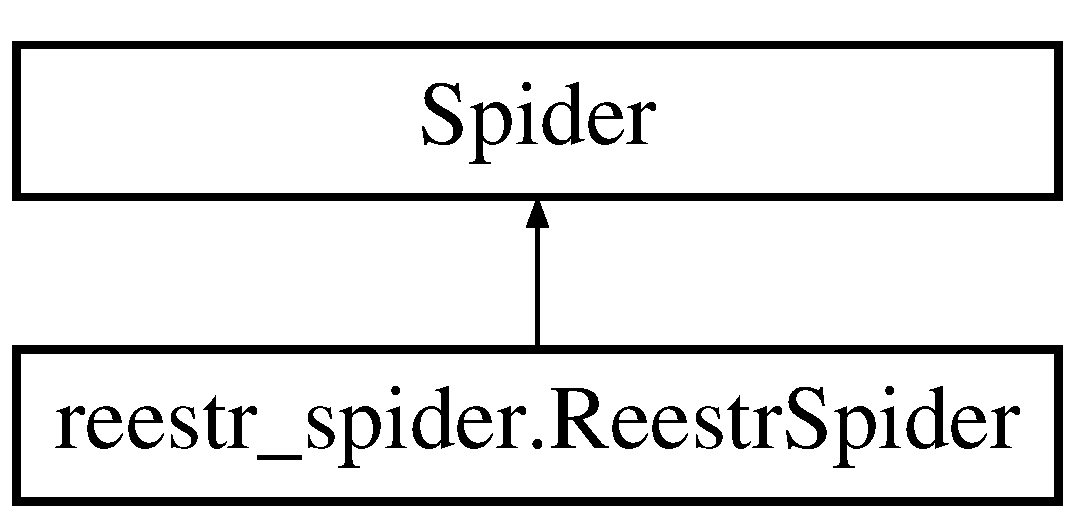
\includegraphics[height=2.000000cm]{classreestr__spider_1_1ReestrSpider}
\end{center}
\end{figure}
\subsection*{Открытые члены}
\begin{DoxyCompactItemize}
\item 
def \hyperlink{classreestr__spider_1_1ReestrSpider_aefeae36f75466e6df09087955be618ff}{start\+\_\+requests} (self)
\begin{DoxyCompactList}\small\item\em Генератор запросов \end{DoxyCompactList}\item 
def \hyperlink{classreestr__spider_1_1ReestrSpider_a1995683a0087b22c906ea7806c1cb3d7}{parse} (self, response)
\begin{DoxyCompactList}\small\item\em Парсер ответа с сервера \end{DoxyCompactList}\end{DoxyCompactItemize}
\subsection*{Открытые статические члены}
\begin{DoxyCompactItemize}
\item 
def \hyperlink{classreestr__spider_1_1ReestrSpider_ac04a7814ce5c2beb13a2ad733cfd49ff}{delete\+\_\+spaces} (line)
\begin{DoxyCompactList}\small\item\em Метод, удаляющий лишние пробельные символы в строке \end{DoxyCompactList}\end{DoxyCompactItemize}
\subsection*{Статические открытые данные}
\begin{DoxyCompactItemize}
\item 
\mbox{\Hypertarget{classreestr__spider_1_1ReestrSpider_aacc299cb0284b8bed690b8326c7a032e}\label{classreestr__spider_1_1ReestrSpider_aacc299cb0284b8bed690b8326c7a032e}} 
string \hyperlink{classreestr__spider_1_1ReestrSpider_aacc299cb0284b8bed690b8326c7a032e}{name} = \char`\"{}reestr\char`\"{}
\begin{DoxyCompactList}\small\item\em Уникальное название, идентифицирующее паука \end{DoxyCompactList}\end{DoxyCompactItemize}


\subsection{Подробное описание}
Класс паука 

Класс, который парсит все страницы реестра, вычленяя необходимые данные с каждой из них 

\subsection{Методы}
\mbox{\Hypertarget{classreestr__spider_1_1ReestrSpider_ac04a7814ce5c2beb13a2ad733cfd49ff}\label{classreestr__spider_1_1ReestrSpider_ac04a7814ce5c2beb13a2ad733cfd49ff}} 
\index{reestr\+\_\+spider\+::\+Reestr\+Spider@{reestr\+\_\+spider\+::\+Reestr\+Spider}!delete\+\_\+spaces@{delete\+\_\+spaces}}
\index{delete\+\_\+spaces@{delete\+\_\+spaces}!reestr\+\_\+spider\+::\+Reestr\+Spider@{reestr\+\_\+spider\+::\+Reestr\+Spider}}
\subsubsection{\texorpdfstring{delete\+\_\+spaces()}{delete\_spaces()}}
{\footnotesize\ttfamily def reestr\+\_\+spider.\+Reestr\+Spider.\+delete\+\_\+spaces (\begin{DoxyParamCaption}\item[{}]{line }\end{DoxyParamCaption})\hspace{0.3cm}{\ttfamily [static]}}



Метод, удаляющий лишние пробельные символы в строке 


\begin{DoxyParams}{Аргументы}
{\em line} & Строка, которую надо изменить \\
\hline
\end{DoxyParams}
\begin{DoxyReturn}{Возвращает}
Очищенная от лишних пробелов строка Этот метод используется для того, чтобы удалять лишние пробелы и символы табуляции, которые могут встретиться в тексте html-\/кода страницы, полученного в ответ от сервера. 
\end{DoxyReturn}
\mbox{\Hypertarget{classreestr__spider_1_1ReestrSpider_a1995683a0087b22c906ea7806c1cb3d7}\label{classreestr__spider_1_1ReestrSpider_a1995683a0087b22c906ea7806c1cb3d7}} 
\index{reestr\+\_\+spider\+::\+Reestr\+Spider@{reestr\+\_\+spider\+::\+Reestr\+Spider}!parse@{parse}}
\index{parse@{parse}!reestr\+\_\+spider\+::\+Reestr\+Spider@{reestr\+\_\+spider\+::\+Reestr\+Spider}}
\subsubsection{\texorpdfstring{parse()}{parse()}}
{\footnotesize\ttfamily def reestr\+\_\+spider.\+Reestr\+Spider.\+parse (\begin{DoxyParamCaption}\item[{}]{self,  }\item[{}]{response }\end{DoxyParamCaption})}



Парсер ответа с сервера 


\begin{DoxyParams}{Аргументы}
{\em response} & Объект класса scrapy.\+http.\+Text\+Response, внутри которого находится содержимое страницы и методы для дальнейшей обработки ответа сервера.\\
\hline
\end{DoxyParams}
Метод, который вызывается для обработки ответа, получаемого после каждого запроса. \mbox{\Hypertarget{classreestr__spider_1_1ReestrSpider_aefeae36f75466e6df09087955be618ff}\label{classreestr__spider_1_1ReestrSpider_aefeae36f75466e6df09087955be618ff}} 
\index{reestr\+\_\+spider\+::\+Reestr\+Spider@{reestr\+\_\+spider\+::\+Reestr\+Spider}!start\+\_\+requests@{start\+\_\+requests}}
\index{start\+\_\+requests@{start\+\_\+requests}!reestr\+\_\+spider\+::\+Reestr\+Spider@{reestr\+\_\+spider\+::\+Reestr\+Spider}}
\subsubsection{\texorpdfstring{start\+\_\+requests()}{start\_requests()}}
{\footnotesize\ttfamily def reestr\+\_\+spider.\+Reestr\+Spider.\+start\+\_\+requests (\begin{DoxyParamCaption}\item[{}]{self }\end{DoxyParamCaption})}



Генератор запросов 

\begin{DoxyReturn}{Возвращает}
Итерируемый объект, содержащий список объектов scrapy.\+Request 
\end{DoxyReturn}


Объявления и описания членов класса находятся в файле\+:\begin{DoxyCompactItemize}
\item 
data\+\_\+mining/spiders/reestr\+\_\+spider.\+py\end{DoxyCompactItemize}

\hypertarget{classUrlsReceiver_1_1UrlsReceiver}{}\section{Класс Urls\+Receiver.\+Urls\+Receiver}
\label{classUrlsReceiver_1_1UrlsReceiver}\index{Urls\+Receiver.\+Urls\+Receiver@{Urls\+Receiver.\+Urls\+Receiver}}


Получатель списка ссылок  


\subsection*{Открытые члены}
\begin{DoxyCompactItemize}
\item 
def \hyperlink{classUrlsReceiver_1_1UrlsReceiver_ae4ba1b935dce3bd30912583beca32aff}{\+\_\+\+\_\+init\+\_\+\+\_\+} (self, main\+\_\+url)
\begin{DoxyCompactList}\small\item\em Конструктор \end{DoxyCompactList}\item 
def \hyperlink{classUrlsReceiver_1_1UrlsReceiver_a448316919bfe59e35942edc34f2b674b}{get\+\_\+html\+\_\+code} (self, url)
\begin{DoxyCompactList}\small\item\em Метод, получающий html-\/кода страницы \end{DoxyCompactList}\item 
def \hyperlink{classUrlsReceiver_1_1UrlsReceiver_ace2cdcb9a1bb117d80ec0efad2b2374b}{get\+\_\+urls\+\_\+from\+\_\+page} (self, page\+\_\+num)
\begin{DoxyCompactList}\small\item\em Метод, собирающий ссылки с одной страницы \end{DoxyCompactList}\item 
def \hyperlink{classUrlsReceiver_1_1UrlsReceiver_a1dfd347420ffce5e3c510feb8a436d30}{make\+\_\+url} (self, url)
\begin{DoxyCompactList}\small\item\em Метод, приводящий в нормальный вид ссылку, полученную из html-\/кода страницы \end{DoxyCompactList}\item 
def \hyperlink{classUrlsReceiver_1_1UrlsReceiver_a871a6b2bc7d65cd8ea6184061f994592}{get\+\_\+max\+\_\+page\+\_\+num} (self)
\begin{DoxyCompactList}\small\item\em Метод, получающий количество страниц в реестре \end{DoxyCompactList}\item 
def \hyperlink{classUrlsReceiver_1_1UrlsReceiver_abf0eed73148dbb302da0b4a09efb4940}{parse\+\_\+reestr} (self)
\begin{DoxyCompactList}\small\item\em Главный метод \end{DoxyCompactList}\end{DoxyCompactItemize}
\subsection*{Открытые атрибуты}
\begin{DoxyCompactItemize}
\item 
\mbox{\Hypertarget{classUrlsReceiver_1_1UrlsReceiver_a26ea003c345156c0e7cdeb49750b15f2}\label{classUrlsReceiver_1_1UrlsReceiver_a26ea003c345156c0e7cdeb49750b15f2}} 
{\bfseries main\+\_\+url}
\item 
\mbox{\Hypertarget{classUrlsReceiver_1_1UrlsReceiver_a4a9800032de527abd7fbc8dfed704d53}\label{classUrlsReceiver_1_1UrlsReceiver_a4a9800032de527abd7fbc8dfed704d53}} 
{\bfseries html\+\_\+code}
\item 
\mbox{\Hypertarget{classUrlsReceiver_1_1UrlsReceiver_afd8cf89e02fd746d77d6074eeacaec0e}\label{classUrlsReceiver_1_1UrlsReceiver_afd8cf89e02fd746d77d6074eeacaec0e}} 
{\bfseries answer}
\item 
\mbox{\Hypertarget{classUrlsReceiver_1_1UrlsReceiver_aa118829b177026eba1f6701b7178fbfb}\label{classUrlsReceiver_1_1UrlsReceiver_aa118829b177026eba1f6701b7178fbfb}} 
{\bfseries urls}
\item 
\mbox{\Hypertarget{classUrlsReceiver_1_1UrlsReceiver_af9f409bb62f37a08c7fc7eb37e07dd2a}\label{classUrlsReceiver_1_1UrlsReceiver_af9f409bb62f37a08c7fc7eb37e07dd2a}} 
{\bfseries page\+\_\+num}
\item 
\mbox{\Hypertarget{classUrlsReceiver_1_1UrlsReceiver_ad10c955c9e74df17b8f5f9cc6a80a5e7}\label{classUrlsReceiver_1_1UrlsReceiver_ad10c955c9e74df17b8f5f9cc6a80a5e7}} 
{\bfseries context}
\end{DoxyCompactItemize}


\subsection{Подробное описание}
Получатель списка ссылок 

Класс, с помощью которого можно получить список ссылок на все российские прораммы для ЭВМ и БД из единого реестра {\ttfamily \href{https://reestr.minsvyaz.ru/reestr/}{\tt https\+://reestr.\+minsvyaz.\+ru/reestr/}} 

\subsection{Конструктор(ы)}
\mbox{\Hypertarget{classUrlsReceiver_1_1UrlsReceiver_ae4ba1b935dce3bd30912583beca32aff}\label{classUrlsReceiver_1_1UrlsReceiver_ae4ba1b935dce3bd30912583beca32aff}} 
\index{Urls\+Receiver\+::\+Urls\+Receiver@{Urls\+Receiver\+::\+Urls\+Receiver}!\+\_\+\+\_\+init\+\_\+\+\_\+@{\+\_\+\+\_\+init\+\_\+\+\_\+}}
\index{\+\_\+\+\_\+init\+\_\+\+\_\+@{\+\_\+\+\_\+init\+\_\+\+\_\+}!Urls\+Receiver\+::\+Urls\+Receiver@{Urls\+Receiver\+::\+Urls\+Receiver}}
\subsubsection{\texorpdfstring{\+\_\+\+\_\+init\+\_\+\+\_\+()}{\_\_init\_\_()}}
{\footnotesize\ttfamily def Urls\+Receiver.\+Urls\+Receiver.\+\_\+\+\_\+init\+\_\+\+\_\+ (\begin{DoxyParamCaption}\item[{}]{self,  }\item[{}]{main\+\_\+url }\end{DoxyParamCaption})}



Конструктор 


\begin{DoxyParams}{Аргументы}
{\em self} & \\
\hline
{\em main\+\_\+url} & Ссылка на первую страницу реестра, с которой потом будет осуществляться переход на остальные страницы \\
\hline
\end{DoxyParams}


\subsection{Методы}
\mbox{\Hypertarget{classUrlsReceiver_1_1UrlsReceiver_a448316919bfe59e35942edc34f2b674b}\label{classUrlsReceiver_1_1UrlsReceiver_a448316919bfe59e35942edc34f2b674b}} 
\index{Urls\+Receiver\+::\+Urls\+Receiver@{Urls\+Receiver\+::\+Urls\+Receiver}!get\+\_\+html\+\_\+code@{get\+\_\+html\+\_\+code}}
\index{get\+\_\+html\+\_\+code@{get\+\_\+html\+\_\+code}!Urls\+Receiver\+::\+Urls\+Receiver@{Urls\+Receiver\+::\+Urls\+Receiver}}
\subsubsection{\texorpdfstring{get\+\_\+html\+\_\+code()}{get\_html\_code()}}
{\footnotesize\ttfamily def Urls\+Receiver.\+Urls\+Receiver.\+get\+\_\+html\+\_\+code (\begin{DoxyParamCaption}\item[{}]{self,  }\item[{}]{url }\end{DoxyParamCaption})}



Метод, получающий html-\/кода страницы 


\begin{DoxyParams}{Аргументы}
{\em self} & \\
\hline
{\em url} & Ссылка на страницу, html-\/код которой необходимо получить\\
\hline
\end{DoxyParams}
html-\/код страницы получается с помощью библиотеки {\ttfamily urllib.\+request}. Далее он записывается в поле {\ttfamily self.\+html\+\_\+code}. \mbox{\Hypertarget{classUrlsReceiver_1_1UrlsReceiver_a871a6b2bc7d65cd8ea6184061f994592}\label{classUrlsReceiver_1_1UrlsReceiver_a871a6b2bc7d65cd8ea6184061f994592}} 
\index{Urls\+Receiver\+::\+Urls\+Receiver@{Urls\+Receiver\+::\+Urls\+Receiver}!get\+\_\+max\+\_\+page\+\_\+num@{get\+\_\+max\+\_\+page\+\_\+num}}
\index{get\+\_\+max\+\_\+page\+\_\+num@{get\+\_\+max\+\_\+page\+\_\+num}!Urls\+Receiver\+::\+Urls\+Receiver@{Urls\+Receiver\+::\+Urls\+Receiver}}
\subsubsection{\texorpdfstring{get\+\_\+max\+\_\+page\+\_\+num()}{get\_max\_page\_num()}}
{\footnotesize\ttfamily def Urls\+Receiver.\+Urls\+Receiver.\+get\+\_\+max\+\_\+page\+\_\+num (\begin{DoxyParamCaption}\item[{}]{self }\end{DoxyParamCaption})}



Метод, получающий количество страниц в реестре 

В переменную {\ttfamily self.\+page\+\_\+num} записывается число страниц в реестре с ссылками на ПО \mbox{\Hypertarget{classUrlsReceiver_1_1UrlsReceiver_ace2cdcb9a1bb117d80ec0efad2b2374b}\label{classUrlsReceiver_1_1UrlsReceiver_ace2cdcb9a1bb117d80ec0efad2b2374b}} 
\index{Urls\+Receiver\+::\+Urls\+Receiver@{Urls\+Receiver\+::\+Urls\+Receiver}!get\+\_\+urls\+\_\+from\+\_\+page@{get\+\_\+urls\+\_\+from\+\_\+page}}
\index{get\+\_\+urls\+\_\+from\+\_\+page@{get\+\_\+urls\+\_\+from\+\_\+page}!Urls\+Receiver\+::\+Urls\+Receiver@{Urls\+Receiver\+::\+Urls\+Receiver}}
\subsubsection{\texorpdfstring{get\+\_\+urls\+\_\+from\+\_\+page()}{get\_urls\_from\_page()}}
{\footnotesize\ttfamily def Urls\+Receiver.\+Urls\+Receiver.\+get\+\_\+urls\+\_\+from\+\_\+page (\begin{DoxyParamCaption}\item[{}]{self,  }\item[{}]{page\+\_\+num }\end{DoxyParamCaption})}



Метод, собирающий ссылки с одной страницы 


\begin{DoxyParams}{Аргументы}
{\em self} & \\
\hline
{\em page\+\_\+num} & Номер страницы реестра, с которой получается список ссылок\\
\hline
\end{DoxyParams}
Внутри метода составлено регулярное выражение, по которому выбираются все ссылки в html-\/коде страницы, после чего записываются в файл {\ttfamily urls.\+txt}. После обработки очередной страницы в стандартный вывод пишется ее номер. \mbox{\Hypertarget{classUrlsReceiver_1_1UrlsReceiver_a1dfd347420ffce5e3c510feb8a436d30}\label{classUrlsReceiver_1_1UrlsReceiver_a1dfd347420ffce5e3c510feb8a436d30}} 
\index{Urls\+Receiver\+::\+Urls\+Receiver@{Urls\+Receiver\+::\+Urls\+Receiver}!make\+\_\+url@{make\+\_\+url}}
\index{make\+\_\+url@{make\+\_\+url}!Urls\+Receiver\+::\+Urls\+Receiver@{Urls\+Receiver\+::\+Urls\+Receiver}}
\subsubsection{\texorpdfstring{make\+\_\+url()}{make\_url()}}
{\footnotesize\ttfamily def Urls\+Receiver.\+Urls\+Receiver.\+make\+\_\+url (\begin{DoxyParamCaption}\item[{}]{self,  }\item[{}]{url }\end{DoxyParamCaption})}



Метод, приводящий в нормальный вид ссылку, полученную из html-\/кода страницы 


\begin{DoxyParams}{Аргументы}
{\em url} & Строка вида {\ttfamily /reestr/123456/} \\
\hline
\end{DoxyParams}
\begin{DoxyReturn}{Возвращает}
Ссылку вида {\ttfamily \href{https://reestr.minsvyaz.ru/reestr/123456}{\tt https\+://reestr.\+minsvyaz.\+ru/reestr/123456}} 
\end{DoxyReturn}
\mbox{\Hypertarget{classUrlsReceiver_1_1UrlsReceiver_abf0eed73148dbb302da0b4a09efb4940}\label{classUrlsReceiver_1_1UrlsReceiver_abf0eed73148dbb302da0b4a09efb4940}} 
\index{Urls\+Receiver\+::\+Urls\+Receiver@{Urls\+Receiver\+::\+Urls\+Receiver}!parse\+\_\+reestr@{parse\+\_\+reestr}}
\index{parse\+\_\+reestr@{parse\+\_\+reestr}!Urls\+Receiver\+::\+Urls\+Receiver@{Urls\+Receiver\+::\+Urls\+Receiver}}
\subsubsection{\texorpdfstring{parse\+\_\+reestr()}{parse\_reestr()}}
{\footnotesize\ttfamily def Urls\+Receiver.\+Urls\+Receiver.\+parse\+\_\+reestr (\begin{DoxyParamCaption}\item[{}]{self }\end{DoxyParamCaption})}



Главный метод 

Метод, после запуска которого последовательно обходятся все страницы с ссылками реестра , с которых в файл {\ttfamily urls.\+txt} записываются ссылки на продукты, каждую из которых впоследствии надо будет обработать и составить {\ttfamily .csv} файл 

Объявления и описания членов класса находятся в файле\+:\begin{DoxyCompactItemize}
\item 
Urls\+Receiver.\+py\end{DoxyCompactItemize}

%--- End generated contents ---

% Index
\backmatter
\newpage
\phantomsection
\clearemptydoublepage
\addcontentsline{toc}{chapter}{Алфавитный указатель}
\printindex

\end{document}
